\chapter{Metodolog\'ia de simulaci\'on de redes de fracturas discretas}
\label{s:dfnModeling}

En este cap\'itulo se muestra de manera esquem\'atica los ingredientes principales de los cap\'itulos anteriores. Para ello, es necesario explicar la manera en que se desarrollar\'an tales ideas principales.

Un diagrama de flujo (flowchart) es una representaci\'on gr\'afica que resalta los elementos de un programa computacional o una metodolog\'ia, las relaciones entre ellos, as\'i como su correspondiente orden de ejecuci\'on (flujo l\'ogico). Para mayor informaci\'on sobre diagramas de flujo su puede consultar los libros de \cite{venit_prelude_2014} y \cite{farrell_programming_2014}.

\begin{table}[H]
	\centering
	\caption{S\'imbolos b\'asicos para construir diagramas de flujo.}
	\label{tab:flowcharCheatsheet}
	\begin{tabular}{|ccl|}
		\hline
		S\'imbolo & Nombre & Descripci\'on \\ \hline
		\tikz \draw (0,0) rectangle (1.5,0.5); & Proceso  & Representa cualquier proceso, c\'alculo \'o funci\'on. \\ \hline
		\tikz \draw (0,0) node[trapezium, trapezium left angle=70, trapezium right angle=110, draw, minimum height=0.5cm] {}; & Input/output & Argumento de entrada o salida. \\ \hline
		\tikz \draw (0,0) node[shape aspect=2,diamond,draw] {}; & Decisi\'on & Representa una decisi\'on binaria, usualmente S\'i o No. \\ \hline
		\tikz \draw (0,0) -- (1,0); & Flecha & Indica la direcci\'on de flujo de control. \\ \hline
	\end{tabular}
\end{table}

Adem\'as, algunos s\'imbolos de la \autoref{tab:flowcharCheatsheet} rellenos con color verde (\tikz \fill[green!30] (0,0) rectangle (0.8,0.3);) representan los inicios de cada diagrama de flujo, mientras que en color rojo (\tikz \fill[red!30] (0,0) rectangle (0.8,0.3);) los finales de los mismos. En el caso de diagramas verticales, el mismo se lee de arriba hacia abajo.

\section{An\'alisis, modelado y simulaci\'on de variables aleatorias}

El enfoque que se utilizar\'a en esta secci\'on es el convencional en ciencias de la tierra en donde, teniendo datos, se procede a caracterizarlos, es decir, a entender su comportamiento en la mayor medida posible. Posteriormente se puede hacer el modelado teniendo en cuenta el paso anterior y posteriormente pueden hacer simulaciones estad\'isticamente equivalentes con los datos. Estos pasos, para el caso univariado, se puede ver reflejado en el diagrama de flujo de la \autoref{f:workflowSim1D}, yendo de lo rojo hacia lo verde.

La caracterizaci\'on se basa principalmente en an\'alisis exploratorio de los datos $x_s$ (en el globo rojo en la \autoref{f:workflowSim1D}). En esta etapa del an\'alisis estad\'istico se analizan individualmente cada una de las propiedades de las fracturas, as\'i como de la red de fracturas. El resultado esperado para esta etapa es entender el fen\'omeno subyacente a los datos, para as\'i poder modelar o sugerir modelos de distribuci\'on de probabilidad para cada una de las propiedades de fractura.

Para lograr este objetivo se hace uso de estad\'igrafos y de gr\'aficas. Por ejemplo, la media proporciona una medida de tendencia centra, mientras que la desviaci\'on est\'andar proporciona informaci\'on sobre qu\'e tan dispersos se encuentran los datos con respecto a la media obtenida. Esto es v\'alido tanto para las longitudes como para las orientaciones, claro, cada variable con su teor\'ia correspondiente. El an\'alisis exploratorio siempre debe de combinar los estad\'igrafos y los gr\'aficos. Para las longitudes se puede utilizar los gr\'aficos de caja y los histogramas principalmente. Para las orientaciones es \'util utilizar las rosetas de orientaciones, pero un histograma resalta m\'as cualquier moda sutil que se escape a la vista en una roseta.

\begin{figure}[H]
	\centering
	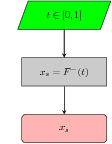
\includegraphics{rvSim}
	\caption{Diagrama de flujo para obtener una simulaci\'on de una variable aleatoria. En este caso puede ser la orientaci\'on o la longitud. Comp\'arese con la \autoref{f:cdf1D}.}
\label{f:workflowSim1D}
\end{figure}

En la siguiente etapa, en color gris en la \autoref{f:workflowSim1D}, se procede a modelar la funci\'on de probabilidad para los datos. Aqu\'i se puede proceder con el enfoque com\'un de hacer pruebas de hip\'otesis para varios modelos propuestos o se puede hacer con el enfoque de los cuantiles de Bernstein-Kantorovich utilizado en este trabajo doctoral.

Para hacer la simulaci\'on, hay que recorrer la \autoref{f:workflowSim1D} en sentido contrario en el que lo hicimos para la caracterizaci\'on y el modelado. Ahora, el algoritmo de simulaci\'on muestra que debemos empezar con un valor simulado $t$ obtenido de una distribuci\'on $Uniforme(0,1)$. La funci\'on cuantil $F^-(t)$ nos proporcionar\'a un valor simulado. De esta manera podemos obtener las simulaciones necesarias para estimar la incertidumbre.

\section{An\'alisis, modelado y simulaci\'on de la estructura de dependencia entre variables aleatorias}

Igual de importante que estudiar individualmente las propiedades de fractura es estudiar la relaci\'on que existen entre tales propiedades. Se recomienda estudiar, primero, las relaciones por pares, es decir de manera bivariada. Dos ejemplos de relaciones bivariadas ser\'ian (1) longitud y apertura, y (2) orientaci\'on y longitud. Posteriormente se puede estudiar de manera trivariada o multivariada pero en estos casos es dif\'icil obtener una idea visual de la estructura de dependencia.

El gr\'afico m\'as \'util para estudiar las dependencias entre variables aleatorias es el gr\'afico o diagrama de pseudo-observaciones. Dicho gr\'afico se forma con las pseudo-observaciones obtenidas a partir de la funci\'on de distribuci\'on emp\'irica (\autoref{e:empF}). Para obtenerlas se presenta el diagrama de flujo en la \autoref{f:pseudoObsWF}. N\'otese que en el diagrama se muestra la funci\'on de distribuci\'on de probabilidad $F(\cdot)$ de manera general, pero en este trabajo se utiliza $F(x)=\hat{F}_n(x)$. Los puntos de cada pseudo-observaci\'on $(u_i, v_i)$, $i \in \{1, \ldots, n\}$ formados con las variables $X$ y $Y$ se grafican en el plano $uv$ (\autoref{fig:pseudoObsPlotGeneration}) para obtener un diagrama de dispersi\'on de las pseudo-observaciones.

\begin{figure}
	\centering
	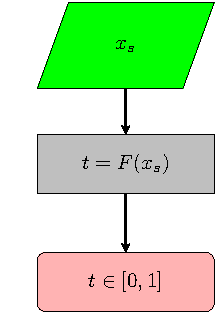
\includegraphics{rvModeling}
	\caption{Diagrama de flujo para obtener las pseudo-observaciones. Comp\'arese con la \autoref{f:cdf1D}.}
\label{f:pseudoObsWF}
\end{figure}


\begin{figure}
	\centering
	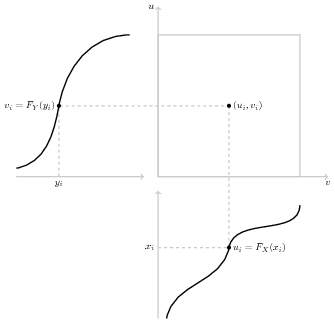
\includegraphics{pseudoObsPlotGeneration}
	\caption{Obtenci\'on del diagrama de pseudo-observaciones con el cual se estudia la dependencia entre dos variables aleatorias. Las funciones de distribuci\'on marginales que se muestran son continuas pero pueden ser no-continuas o una combinaci\'on de ambas.}
	\label{fig:pseudoObsPlotGeneration}
\end{figure}

Dentro del contexto de la teor\'ia de c\'opulas el comportamiento conjunto queda totalmente determinado por la c\'opula, y de manera casi directa por las pseudo-observaciones. Una manera de facilitar el an\'alisis del gr\'afico de pseudo-observaciones es agregando una sub-capa tipo mosaico o pixeles. Un ejemplo muy sencillo se muestra en el recuadro derecho de la \autoref{f:dependenceAnalysis1}. Se propone, como primer paso, que la sub-capa sea determinada por los cuartiles y los valores m\'aximos y m\'inimos de los datos. En particular se propone que los cuartiles se calculen a partir de los modelos de los datos ya que de esta manera se pueden comparar diversas simulaciones sobre un mismo mosaico. En el ejemplo de la \autoref{f:dependenceAnalysis1} se tiene que $q_{1X} = F_X^-(0.25)$, $M=F_Y^-(0.5)$.

\begin{figure}[H]
	\centering
	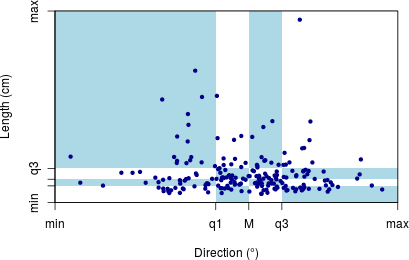
\includegraphics[width=0.4\textwidth]{bivariateInd-15}
	\qquad
	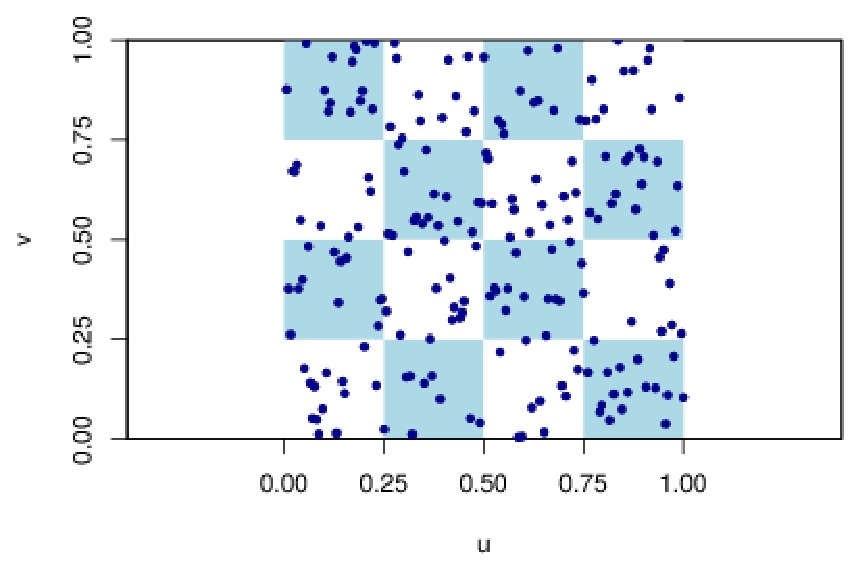
\includegraphics[width=0.4\textwidth]{bivariateInd-14}
	\caption{Diagrama de dispersi\'on con m\'ultiples zonas remarcadas a fin de hacer un an\'alisis exploratorio preliminar.}
	\label{f:dependenceAnalysis2}
\end{figure}

Aunque la c\'opula tiene la informaci\'on de la estructura de dependencia, conviene graficar tambi\'en el diagrama de dispersi\'on de los datos ya que ellos, a diferencia de las pseudo-observaciones, est\'an en el rango real. N\'otese que los cuadros del gr\'afico de pseudo-observaciones se extienden o encogen en el diagrama de dispersi\'on, incluso de forma diferente dependiendo el mosaico/pixel (intervalo bidimensional). En la \autoref{f:dependenceAnalysis2} se muestra otro mosaico para otro conjunto de datos debido a que se quiere resaltar que la estructura de dependencia general se puede descomponer en dos estructuras m\'as simples.

\begin{figure}[H]
	\centering
	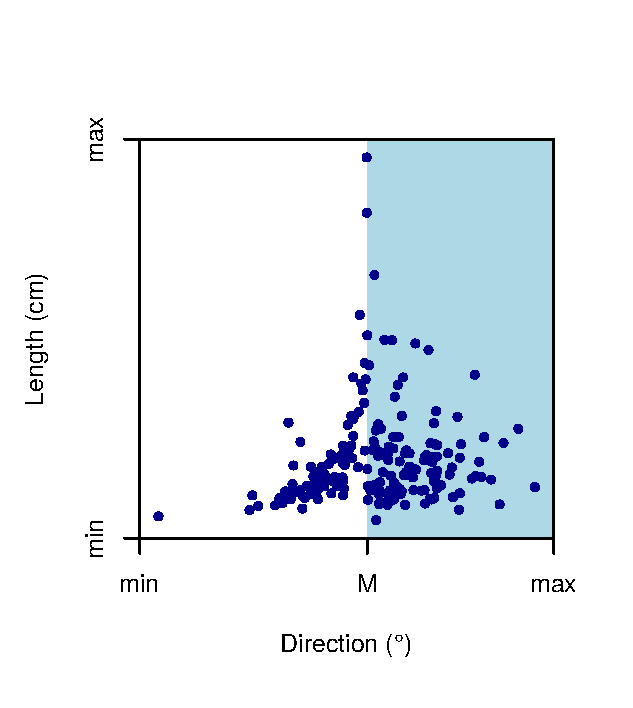
\includegraphics[width=0.4\textwidth]{bivariateDep-24}
	\qquad
	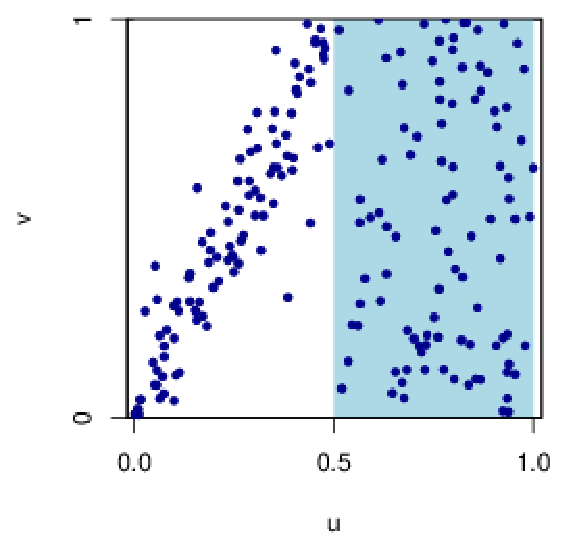
\includegraphics[width=0.4\textwidth]{bivariateDep-26}
	\caption{Diagrama de dispersi\'on en el cual se han resaltado dos zonas con dependencias m\'as simples.}
	\label{f:dependenceAnalysis1}
\end{figure}

% AED: quantitative
De manera cuantitativa, se pueden estimar coeficientes de correlaci\'on y/o hacer pruebas de hip\'otesis sobre la independencia de los datos. Tambi\'en es \'util agregar estos valores al gr\'afico combinado (de dispersi\'on y pseudo-observaciones) ya sea en el gr\'afico o en el pie de figura.

Para la modelaci\'on de la c\'opula bivariada, dentro del contexto de las c\'opulas de Bernstein, se procede a un diagrama de flujo similar al de la \autoref{f:workflowSim1D}. Se analizan los pares de pseudo-observaciones obtenidas mediante la \autoref{f:pseudoObsWF}. \'Estas son inspeccionadas visualmente en un diagrama de dispersi\'on, y cuantitativamente con estad\'igrafos (coeficientes de correlaci\'on \'o asociaci\'on) para determinar si existe o no alguna estructura de dependencia que se deba tomar en cuenta. Si hay dependencia, entonces se modela la c\'opula emp\'irica $\hat{C}_n$ con la cual se ajusta la c\'opula estimada $C$.

\begin{figure}
	\centering
	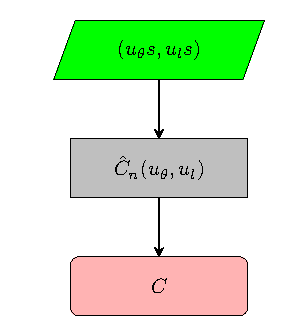
\includegraphics{cop2Dmodeling}
	\caption{Modelaci\'on de la c\'opula a partir de las pseudo-observaciones.}
	\label{f:cop2Dmodeling}
\end{figure}

\section{Diagrama de flujo para el an\'alisis, modelado y simulaci\'on de redes de fracturas discretas tomando en cuenta su estructura de dependencia}

Resulta ilustrativo el diagrama de flujo  de la \autoref{f:rvSim2D} en la modelaci\'on del vector aleatorio bivariado que representa las propiedades de los objetos booleanos en el cual se parte a partir de los datos observados $\theta_i$ y $l_i$. Se han escogido estos s\'imbolos para hacer la analog\'ia con la orientaci\'on y la longitud de fracturas, pero el diagrama de flujo es v\'alido para cualquier par de variables aleatorias continuas.

\begin{figure}[H]
	\centering
	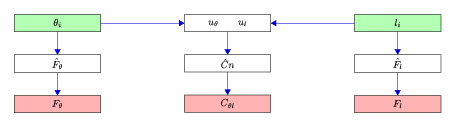
\includegraphics{rvSim2D}
	\caption{Modelaci\'on bivariada de propiedades de objetos booleanos.}
	\label{f:rvSim2D}
\end{figure}

N\'otese que, de arriba hacia abajo, se procede con la caracterizaci\'on de los datos hasta llegar al modelo, en lo parte inferior, tanto de manera univariada como bivariada. En la parte univariada en los extremos izquierdo y derecho del diagrama son los casos particulares del inverso de la metodolog\'ia en la \autoref{f:workflowSim1D}. Si el diagrama en cuesti\'on se recorre en sentido contrario a las l\'ineas de flujo, entonces se obtiene el algoritmo de simulaci\'on bivariado.

\begin{figure}[H]
\begin{center}
\begin{tikzpicture}[scale=1, transform shape]
	\node[trapezium, trapezium left angle=70, trapezium right angle=110,draw, fill=green!30] (n1) at (0,0) {$\mathbf{X}:=\emptyset$};
	\node[draw,below of=n1] (n2) {$n \sim Poisson(\theta |A|)$};
	\node[draw,below of=n2] (n3) {$\forall i \in \{1,\ldots,n\}, \quad \mathbf{x}_i \sim Uniforme(A)$};
	\node[trapezium, trapezium left angle=70, trapezium right angle=110,draw, fill=red!30, below of=n3] (n4) {$\mathbf{X}$};
	\draw (n1)--(n2);
	\draw (n2)--(n3);
	\draw (n3)--(n4);
\end{tikzpicture}
\end{center}
\caption{Diagrama de flujo para obtener ubicaciones espaciales a trav\'es de un proceso puntual. Desde el punto de vista computacional,  la parte superior del diagrama indica crear un arreglo vac\'io que almacene las coordenadas de todos los vertores $\mathbf{x}_i$.}
\label{fig:ppWF}
\end{figure}

Estos dos \'ultimos diagramas de flujo forman la esencia del algoritmo de simulaci\'on de redes de fracturas. Con el algoritmo de la \autoref{f:rvSim2D} se generan los objetos, es decir la orientaci\'on, longitud, etc. de las fracturas; mientras que con el diagrama de la \autoref{fig:ppWF} se obtienen sus ubicaciones espaciales.

El flujo de trabajo est\'andar (\autoref{f:dfnWorkflow}) puede ser siendo utilizado en la parte que corresponde al cluster an\'alisis para determinar familias, el tama\~no de las familias, la direcci\'on y su dispersi\'on, ya que este an\'alisis proporciona informaci\'on valiosa para el entendimiento del sistema geol\'ogico, sin embargo, la modelaci\'on resulta m\'as compatible con los datos si se hace de manera total, ya que no se crean los artificios generados al segmentar bruscamente las familias mediante un valor de corte. Adem\'as, entre mayor sea la cantidad de datos, mejor es la modelaci\'on de funciones de probabilidad.

Con respecto a las caracter\'isticas multivariadas en color azul, es claro que s\'i hay que hacer un an\'alisis basado en la teor\'ia de c\'opulas a como se mostr\'o en la secci\'on pasada. Ya que el enfoque individualista no puede producir relaciones de dependencia que se pueden observar en los sistemas de fracturas reales. \'Este es el aporte principal al conocimiento que se hace con este trabajo de investigaci\'on, en particular la posibilidad para modelar datos orientados y otras propiedades como longitud o apertura.

\begin{figure}[H]
	\centering
	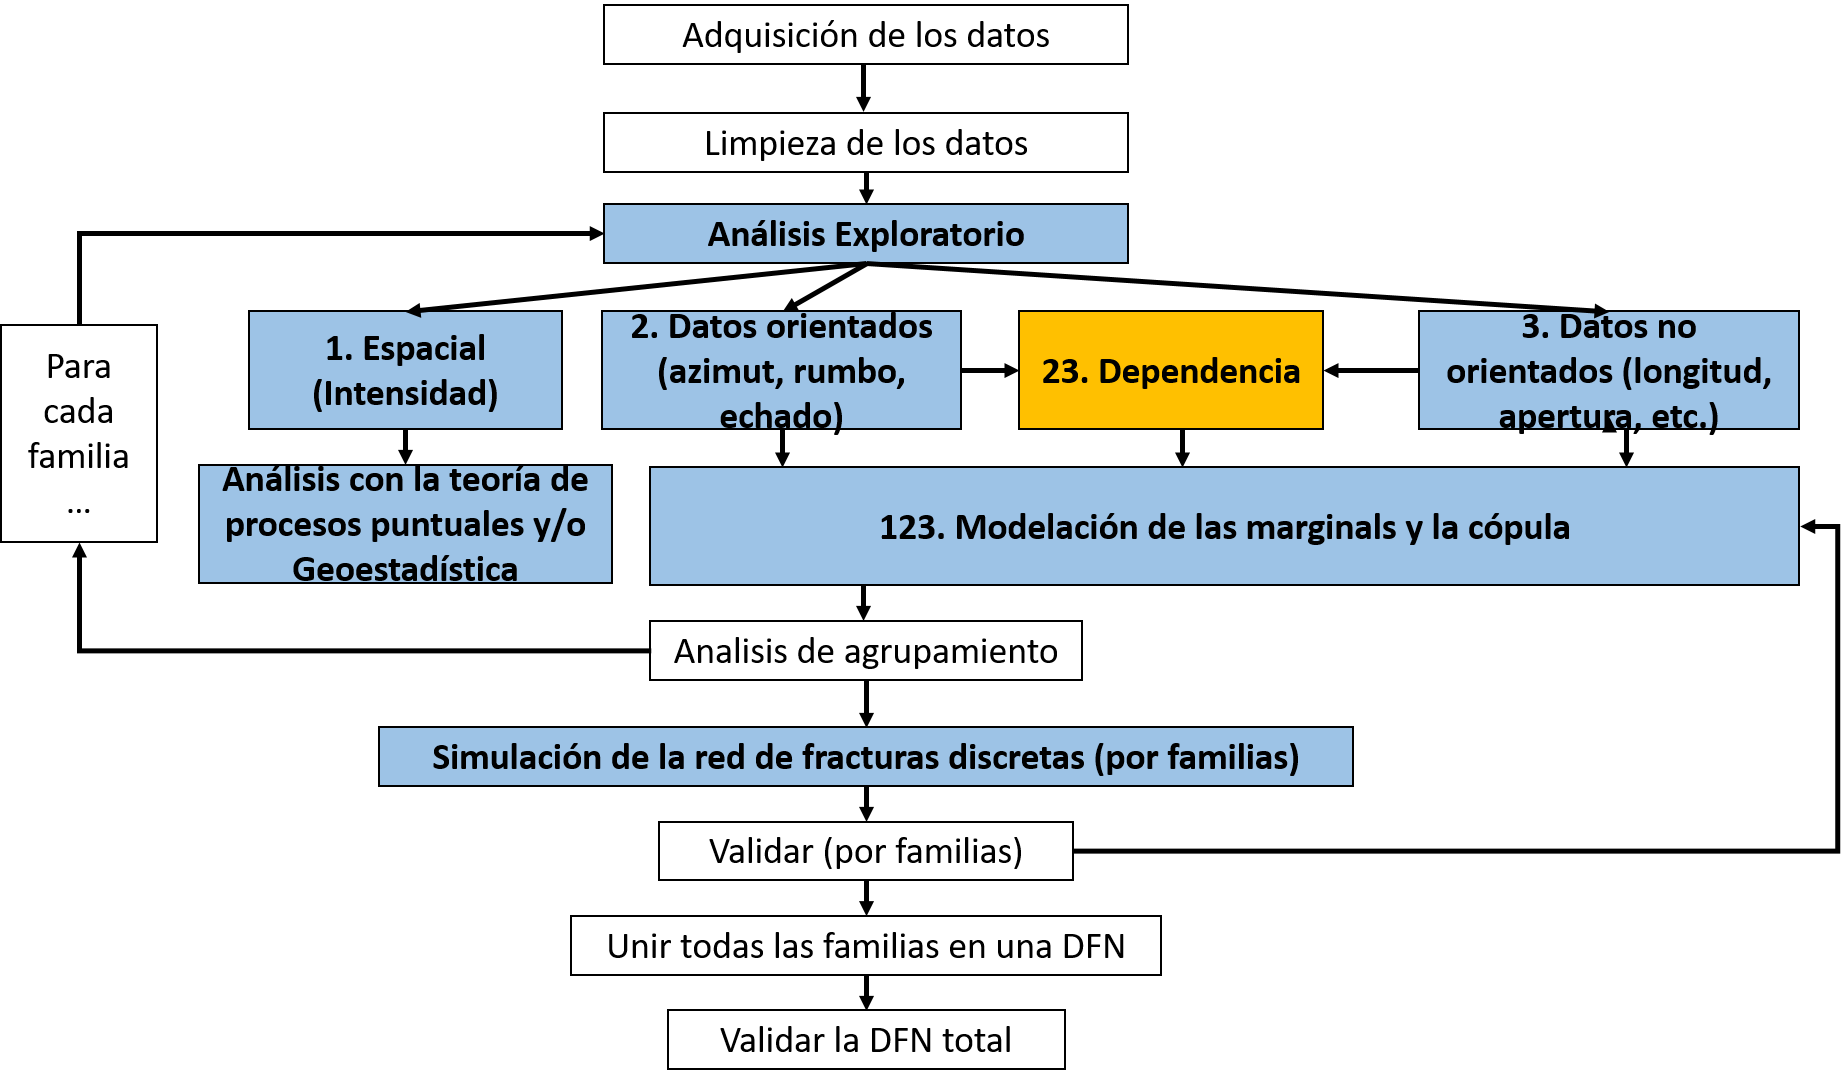
\includegraphics[width=0.8\textwidth]{workflow}
\caption{Flujo de trabajo para la caracterizaci\'on, modelado y simulaci\'on de redes de fracturas discretas en medios porosos fracturados.}
	\label{f:dfnWorkflow}
\end{figure}

El flujo de trabajo (\autoref{f:dfnWorkflow}) comienza en la parte superior con la adquisici\'on de los datos, posteriormente hay que limpiarlos para poder hacer un an\'alisis exploratorio, el cual se realiza de manera univariada (intensidad, orientaci\'on, longitud, apertura, ...) y de manera bivariada se estudian las propiedades mediante las pseudo-observaciones. Como resultado hasta este momento se pudo haber identificado grupos/clusters, los cuales se pueden separar para comenzar el ciclo desde al an\'alisis exploratorio para cada uno de los grupos. Posteriormente se ajustan modelos a cada una de las variables y de manera conjunta con c\'opulas. Estos modelos permiten las simulaciones de fracturas por familias, las cuales tienen que ser validadas, nuevamente, mediante otro an\'alisis exploratorio para verificar que cumple con las mismas propiedades estad\'isticas que los datos. Ahora ya se pueden integrar todas las familias y para finalmente validar la familia global.

Cabe mencionar que el an\'alisis de dependencia tambi\'en puede ayudar para clasificar familias que se distingan de manera bivariada una de otra. Es decir, tambi\'en se puede integrar el an\'alisis de dependencia a cada una de las familias obtenida con el an\'alisis de clusters.

